\section{The \flare\, Simulations}\label{sec:simulations}
\begin{figure*}
	\centering
	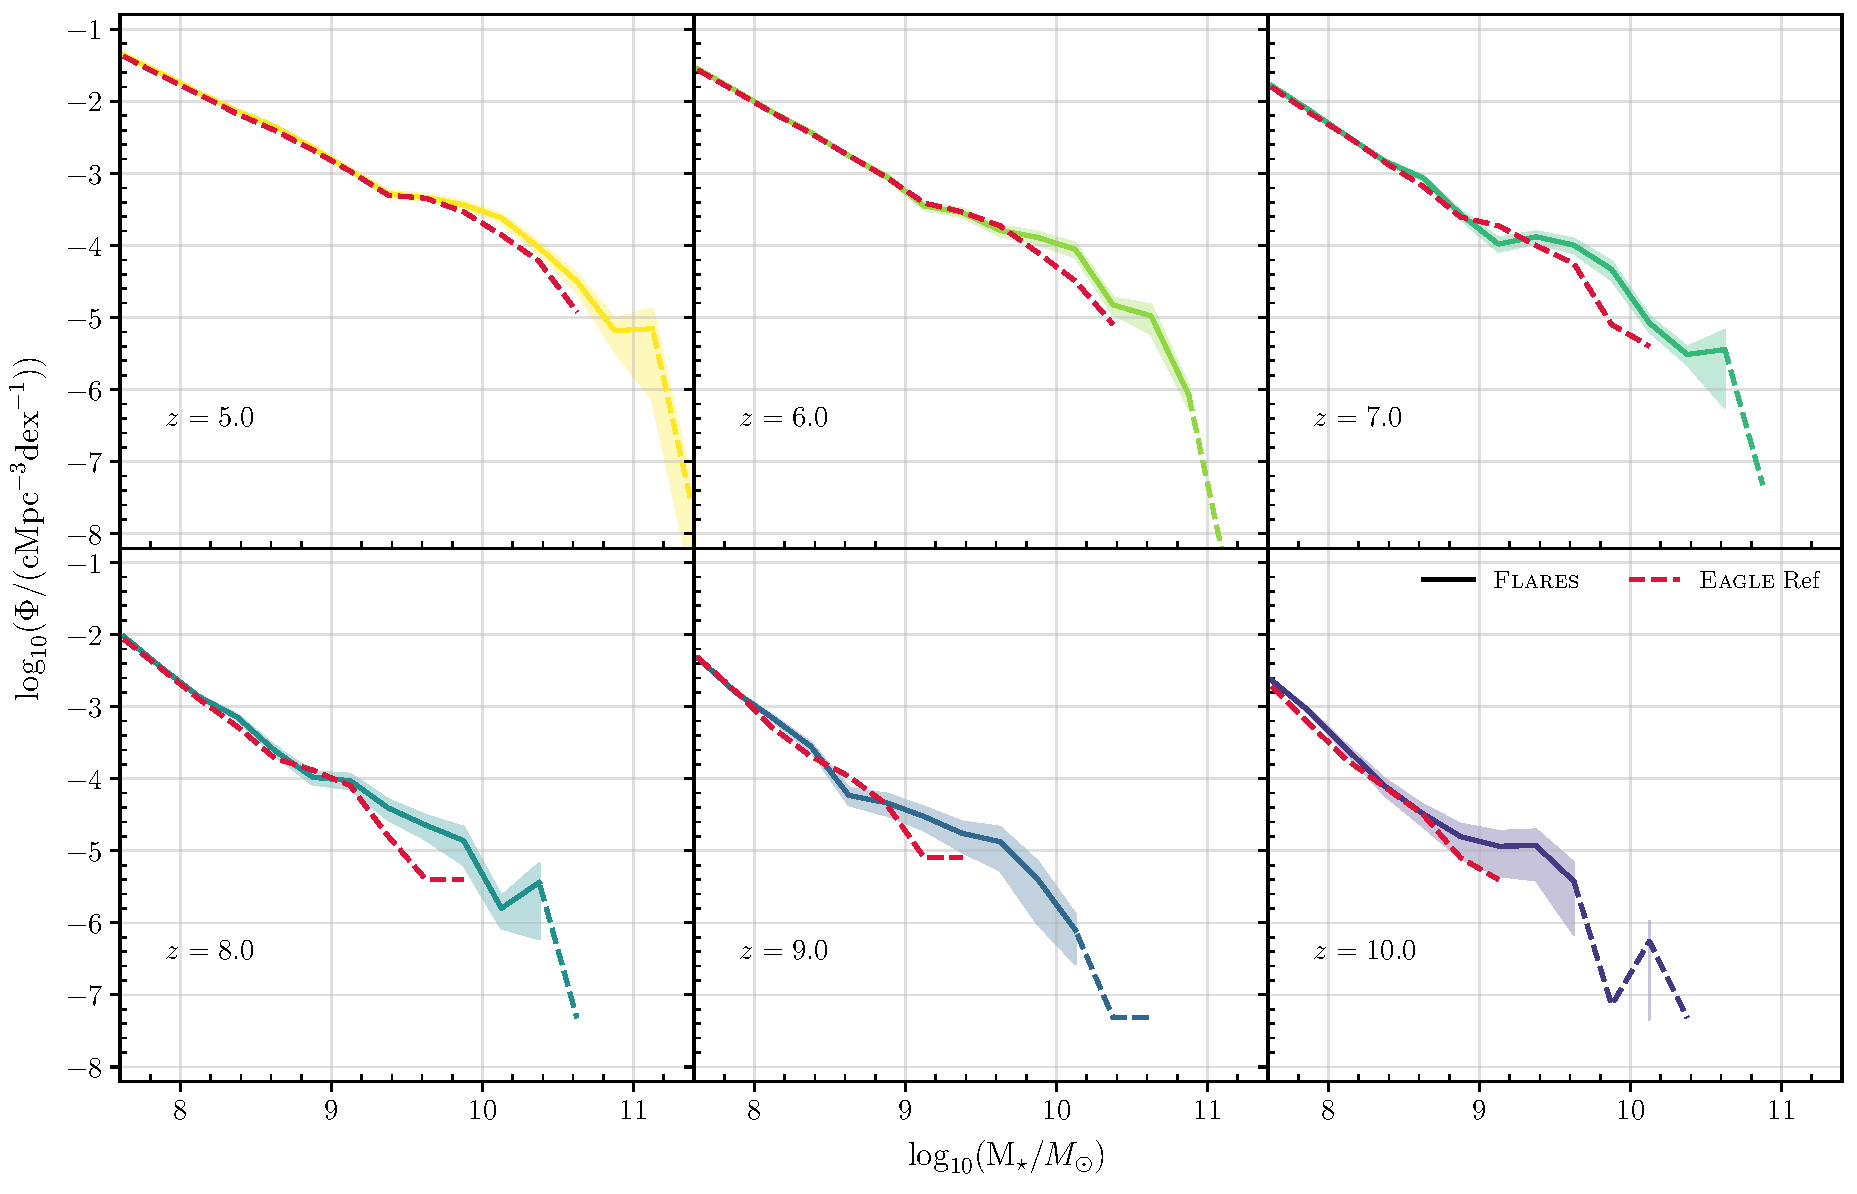
\includegraphics[width=\textwidth]{./figures/GSMF_z5_10}
	\caption{\flares\, composite galaxy stellar mass function (black solid, dashed for bins with less than 3 galaxies) for z $\in$ [5,10]. Shaded region denote the poisson $1\sigma$ uncertainties for	each bin from the simulated number counts for the \flares\, galaxies. For comparison the GSMF from the 100Mpc \eagle\, Reference simulation box is shown. \label{fig: GSMF}} 
\end{figure*}

\textsc{Flares} is a suite of zoom simulations targetting regions with a range of overdensities in the Epoch of Reionisation (EoR). 
These regions are drawn from the same 3.2Gpc a side dark matter only, parent simulation box used in the \ceagle\, simulations \cite{barnes_redshift_2017}. These regions are then re-simualated with full hydrodynamics using the AGNdT9 configuration of the \eagle\, simulation physics as described in \cite{schaye_eagle_2015,crain_eagle_2015}. The simulations have an identical resolution to the 100Mpc Eagle Reference simulation box, with dark matter and an intial gas particle mass of m$_{\text{dm}}=9.7\times10^6$M$_{\odot}$ and m$_{\textrm{g}}=1.8\times10^6$M$_{\odot}$ respectively, and a gravitational softening length of 2.66ckpc. 

\eagle\,, is a series of cosmological simualtions, run with a heavily modified version of \textsc{P-Gadget-3} \citep{springel_simulations_2005}, a N-Body Tree-PM smoothed particle hydrodynamics (SPH) code. The model uses the hydrodynamic solver collectively known as \textsc{Anarchy} \citep[described in][]{schaye_eagle_2015,Schaller2015}, that adopts the pressure-entropy formulation described by \cite{Hopkins2013}, an artificial viscosity switch \citep{cullen_inviscid_2010}, an artificial conduction switch \citep[\eg][]{price_modelling_2008}. The model includes radiative cooling and photo-heating \citep{Wiersma2009a}, star formation \citep{Schaye2008}, stellar evolution and mass loss \citep{Wiersma2009b}, black hole growth \citep{springel_simulations_2005} and feedback from star formation and
AGN \citep{DallaVecchia2012}. The subgrid model was calibrated to reproduce the observed $z=0$ galaxy mass function, the mass-size relation for discs. The model has also been found to be in good agreement with observations of distribution functions at high redshift such as the stellar mass function and the star formation rate function \citep{furlong_evolution_2015}. The AGNdT9 configuration produces similar mass functions to the reference model but better reproduces the hot gas properties in groups and clusters \citep{barnes_cluster-eagle_2017}. It uses a higher value for C$_{\text{visc}}$, a parameter for the effective viscosity of the subgrid accretion, and a higher gas temperature increase from AGN feedback, $\Delta$T. 

The selection of regions from the parent box is done at $z=4.67$, the highest redshift snapshot available for this simulation, from which we select 40 spherical regions with a radius of 14\hMpc\, spanning a wide range of overdensities, ranging from overdensity value of $\delta=-0.479\to0.970$ (shown in Table A1 of \citetalias{lovell2020}). This redshift selection also automatically ensures that the extreme overdensities are mildly non-linear, and thus more or less preserves the rank ordering of overdensities at higher redshifts. We have deliberately selected a greater number of extreme overdensity regions (16) to obtain a large sample of the first massive galaxies that form in the Universe. We also select a number of regions with intermediate and mean overdensities as well as a few underdense regions to better sample the density space and explore the impact of environment on galaxy formation and evolution. 

In order to obtain a representative sample of the Universe, these regions are combined using appropriate weightings, with the very overdense and underdense regions contributing the least to the total weight, thus compensating for any oversampling of the overdense regions. With this weighting technique, we are able to probe a bigger volume without drastically lowering the resolution. For a full description of the simulation and weighting method we refer the readers to \citetalias{lovell2020}.

\subsection{Galaxy Identification}\label{sim.galident}

Galaxies in \flares\,, similar to the standard \eagle\, analysis are identified with \textsc{Subfind} \citep{springel_populating_2001} algorithm within bound groups found from the Friends-Of-Friends \citep[FOF,][]{davis_evolution_1985} algorithm. The stellar masses are defined using star particles identified with \textsc{Subfind} within a 30pkpc aperture centred around the most bound particle of the substructure. In this work we concentrate on a broader definition of a galaxy with respect to \citetalias{lovell2020} focusing on only those objects with a combined total of more than 100 gas and star particles. This extends the stellar mass function down to $\sim$ 10$^{7.5}$\Msun\, at $z=5$. 

\flares\, have more than $\sim$20 times the number of galaxies greater than 10$^{10}$ \Msun\ at $z=5$ compared to the \eagle\, reference volume \citep{schaye_eagle_2015} in the combined volume we resimulate \citepalias[see Figure~5 in][]{lovell2020}. In Figure~\ref{fig: GSMF} we compare the galaxy stellar mass function of the galaxies in \flares\, and the 100Mpc \eagle\, Reference simulation box. It can be seen that \flares\, extends the range by at least an order of magnitude at the high mass end compared to \eagle\,. We explore the results, presenting the various galaxy observables in the coming sections.


\subsection{Spectral Energy Distribution Modelling}\label{sec:simulations.SED}

We broadly follow the approach implemented by \cite{Wilkins2016a,Wilkins2017,Wilkins2018,Wilkins2020} albeit with modifications to the dust modelling as described in \S\ref{sec:modelling.dust}.

\subsubsection{Stellar Emission}

We begin by modelling the pure stellar emission produced by each galaxy. To do this we associate each star particle with a stellar SED according to its age and metallicity (i.e. a simple stellar population or SSP). Throughout this work we utilise v2.2.1 of the Binary Population and Spectral Synthesis (BPASS) stellar population synthesis (SPS) models (reference) and assume a Chabrier initial mass function (IMF) throughout \citep{chabrier_galactic_2003}. As explored in (my photometry paper, my emission line paper, my ionisiing production efficiency paper) the choice of SPS and IMF can have a large effect on resulting broadband luminosities and emission line quantities.

\subsubsection{Nebular Emission}

Young stellar populations produced significant Lyman-continuum (LyC) emission. To account for the reprocessing of these photons by surrounding gas we associate each young ($t<10$ Myr) star particle with a surrounding H{\sc ii} region (or birth cloud) powered by its LyC emission. To calculate the nebular emission we follow the approach detailed in \cite{Wilkins2020}. In short the pure stellar spectrum of each star particle is input to use the {\sc cloudy} (ref, make sure correct version v17.01 I believe?) photo-ionisation code. The metallicity of the associated H{\sc ii} is assumed to be identical to the star particle and we adopt the same dust depletion factors and relative abundances as \cite{Gutkin2016}. We assume a reference (defined at $t=1$ Myr and $Z=0.02$) ionisation parameter of $\log_{10}U_{S,{\rm ref}}=-2$, a hydrogen density of $\log_{10}(n_{H}/{\rm cm^{-3}})=2.5$, and adopt {\sc cloudy}'s default implementation of Orion-type graphite and silicate grains.



